\pdfminorversion=3
\documentclass[tikz,border={0mm 8mm 2mm 0mm}]{standalone}
\usepackage{vuiprepstandalone}
\usepackage{alain2}
\usepackage{pifont}
%\newcommand{\cmark}{\ding{51}}%
%\newcommand{\xmark}{\ding{55}}%
\def\pathfig{CHAP3/ex_Shell/images/}
\usetikzlibrary{decorations,calc}
\usepackage[locale=FR]{siunitx}

\begin{document}

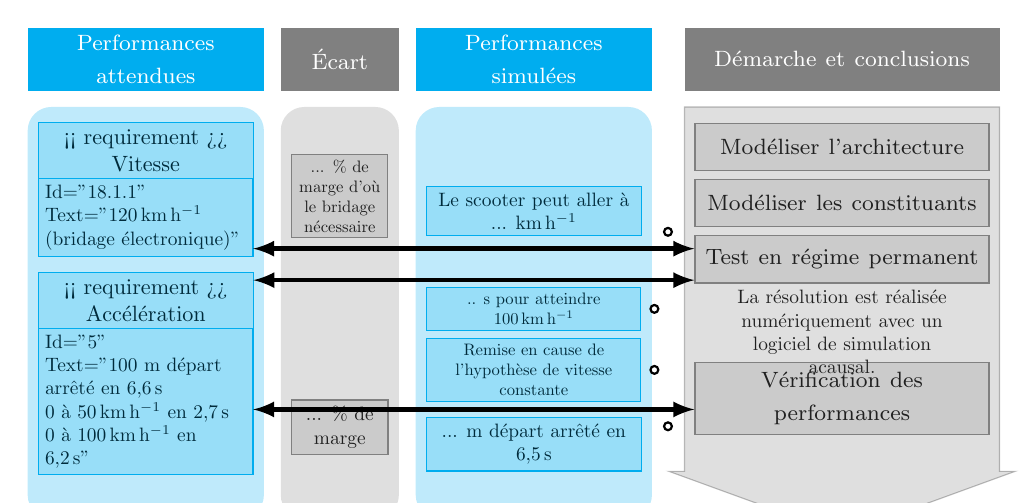
\begin{tikzpicture}

\begin{scope}
\node[white,fill=cyan,align=center,text width=3cm-4pt,inner sep=2pt,minimum height=.8cm] (a) {\footnotesize Performances\\ attendues}; 
%%% A COMPLETER AVEC LES NOEUDS VOULUS
\node[anchor=north,draw=cyan,fill=cyan!20,,rectangle,outer sep=0pt,align=center,text width={(2.5cm+1em/3)/.8-1em/3*.8},scale=.8] (adebut) at ($(a.south)+(0,-.4)$)  {<< requirement >> \\  Vitesse};
\node[anchor=north,draw=cyan,fill=cyan!20,,rectangle,outer sep=0pt,align=left,text width={(2.5cm+1em/3)/.7-1em/3*.7},align=left,scale=.7] (adebut2) at (adebut.south)  {Id="18.1.1"\\ Text="\SI{120}{km.h^{-1}} (bridage électronique)"};


\node[anchor=north,draw=cyan,fill=cyan!20,,rectangle,outer sep=0pt,align=center,text width={(2.5cm+1em/3)/.8-1em/3*.8},scale=.8] (afin0) at ($(adebut2.south)+(0,-.2)$)   {<< requirement >> \\ Accélération};
\node[anchor=north,draw=cyan,fill=cyan!20,rectangle,outer sep=0pt,text width={(2.5cm+1em/3)/.7-1em/3*.7},align=left,scale=.7] (afin) at (afin0.south)  {Id="5"\\ Text="100 m départ arrêté en \SI{6.6}{s}\\
0 à \SI{50}{km.h^{-1}} en \SI{2.7}{s}\\
0 à \SI{100}{km.h^{-1}} en \SI{6.2}{s}"};


\end{scope}

\begin{scope}
\node[white,fill=gray,align=center,text width=1.5cm-4pt,inner sep=2pt,minimum height=.8cm,anchor=west,xshift=.2cm]  (b) at (a.east) {\footnotesize \'Ecart}; 
%%% A COMPLETER AVEC LES NOEUDS VOULUS
\node[text width={(1cm+1em/3)/.6-1em/3*.6},scale=.6,anchor=north,,draw=gray,fill=gray!20,align=center,rectangle] (bdebut) at ($(b.south)+(0,-.8)$)   {... \% de marge d'où le bridage nécessaire};
\node[text width={(1cm+1em/3)/.7-1em/3*.7},scale=.7,anchor=north,,draw=gray,fill=gray!20,align=center,rectangle] (bfin) at ($(bdebut.south)+(0,-2.05)$)   {... \% de marge  };
\end{scope}

\begin{scope}
\node[white,fill=cyan,align=center,text width=3cm-4pt,inner sep=2pt,minimum height=.8cm,anchor=west,xshift=.2cm]  (c) at (b.east) {\footnotesize Performances \\ simulées}; 
%%% A COMPLETER AVEC LES NOEUDS VOULUS
\node[text width={(2.5cm+1em/3)/.7-1em/3*.7},scale=.7,anchor=north,draw=cyan,fill=cyan!20,rectangle,text badly centered] (cdebut) at ($(c.south)+(0,-1.2)$)   {Le scooter peut aller à ... \si{km.h^{-1}}};
\node[text width={(2.5cm+1em/3)/.6-1em/3*.6},scale=.6,anchor=north,draw=cyan,fill=cyan!20,rectangle,text badly centered] (c2) at ($(cdebut.south)+(0,-.65)$)   {.. s pour atteindre \SI{100}{km.h^{-1}}};
\node[text width={(2.5cm+1em/3)/.6-1em/3*.6},scale=.6,anchor=north,draw=cyan,fill=cyan!20,rectangle,text badly centered] (c3) at ($(c2.south)+(0,-.1)$)   {Remise en cause de l'hypothèse de vitesse constante};
\node[text width={(2.5cm+1em/3)/.7-1em/3*.7},scale=.7,anchor=north,draw=cyan,fill=cyan!20,rectangle,text badly centered] (cfin) at ($(c3.south)+(0,-.2)$)   {... m départ arrêté en \SI{6.5}{s} };
\end{scope}

\begin{scope}
\node[white,fill=gray,align=center,text width=4cm-4pt,inner sep=2pt,minimum height=.8cm,anchor=west,xshift=.4cm]  (d) at (c.east) {\footnotesize Démarche et conclusions}; 
%%% A COMPLETER AVEC LES NOEUDS VOULUS
\node[text width=3.5cm,anchor=north,draw=gray,fill=gray!20,rectangle,minimum height=.6cm, align=center] (ddebut) at ($(d.south)+(0,-.4)$)   {\footnotesize Modéliser l'architecture };
\node[text width=3.5cm,anchor=north,draw=gray,fill=gray!20,rectangle,minimum height=.6cm, align=center] (d2) at ($(ddebut.south)+(0,-.1)$)   {\footnotesize Modéliser les constituants };
\node[text width=3.5cm,anchor=north,draw=gray,fill=gray!20,rectangle,minimum height=.6cm, align=center] (d3) at ($(d2.south)+(0,-.1)$)   {\footnotesize Test en régime permanent};
\node[text width=3.5cm,anchor=north,draw=gray,rectangle,fill=gray!20,align=center,minimum height=0cm] (dfin) at ($(d3.south)+(0,-1)$)   {\footnotesize Vérification des performances};
\node[text width=4.5cm,scale=.7,anchor=north,text badly centered] at (d3.south) {La résolution est réalisée numériquement avec un logiciel de simulation acausal.};
\end{scope}

%%% OVERLAY DE LA FIN
%%%%
\coordinate (ymin) at ($(cfin.south)+(0,0)$);
\coordinate (ymax) at ($(adebut.north)$);

\draw[rounded corners = .3cm,draw=none, fill=cyan, opacity=.25, remember picture, overlay] ($(afin.south)!(ymax)!(afin.north)+(-1.5,.2)$) rectangle ($(afin.south)!(ymin)!(afin.north)+(1.5,-.6)$);
\draw[rounded corners = .3cm,draw=none, fill=gray, opacity=.25, remember picture, overlay] ($(bfin.south)!(ymax)!(bfin.north)+(-.75,.2)$) rectangle ($(bfin.south)!(ymin)!(bfin.north)+(.75,-.6)$);
\draw[rounded corners = .3cm,draw=none, fill=cyan, opacity=.25, remember picture, overlay] ($(cfin.south)!(ymax)!(cfin.north)+(-1.5,.2)$) rectangle ($(cfin.south)!(ymin)!(cfin.north)+(1.5,-.6)$);
%\draw[rounded corners = .3cm,draw=none, fill=gray, opacity=.25, remember picture, overlay] ($(ddebut.north)+(-2.,.2)$) rectangle ($(dfin.south)!(ymin)!(dfin.north)+(2.,-.2)$);
\draw[draw=black, fill=gray, opacity=.25, remember picture, overlay] ($(dfin.south)!(ymax)!(dfin.north)+(-2.,.2)$) |- ($(dfin.south)!(ymin)!(dfin.north)+(160:2.341)+(0,-.8)$) -- ++(-20:2.341) -- ++(20:2.341) -| ($(dfin.south)!(ymax)!(dfin.north)+(2.,.2)$) -- cycle;
%%% FLECHE DE FIN
\draw[ultra thick,<->,>=latex] ($(adebut2.south east)+(0,.1)$) -- ($(dfin.west)!($(adebut2.south east)+(0,.1)$)!(ddebut.west)$) node[above,draw, circle,inner sep=1pt,thick,pos=.94,yshift=1.5mm] {\footnotesize\cmark};
\draw[ultra thick,<->,>=latex] ($(afin.east)+(0,-.1)$) -- ($(dfin.west)!($(afin.east)+(0,-.1)$)!(ddebut.west)$) node[below,draw, circle,inner sep=1pt,thick,pos=.94,yshift=-1.5mm] {\footnotesize\cmark};
\draw[ultra thick,<->,>=latex] ($(afin0.north east)+(0,-.1)$) -- ($(dfin.west)!($(afin0.north east)+(0,-.1)$)!(ddebut.west)$);

\node[right,draw, circle,inner sep=1pt,thick,xshift=3pt] at (c2.east)  {\footnotesize\cmark};
\node[right,draw, circle,inner sep=1pt,thick,xshift=3pt] at (c3.east)  {\footnotesize\xmark};
\end{tikzpicture}

\end{document}